\graphicspath{ {./root/4.Annex/2.AnnexIvanInspectionImages/} }

\subsubsection{Evaluator 2 inspection scores}

\begingroup
\setlength{\tabcolsep}{1.5cm}
\renewcommand{\arraystretch}{1.45}

\rowcolors{2}{lightgray}{lightblue}
\begin{longtable}{l r}
	
	\hiderowcolors
	\textbf{Heuristic} & \textbf{Score} \\ \hline  \endhead \\
	\showrowcolors
	
	H1. Visibility of system status & 1  \\
	H2. Match between system and the real world & 5  \\
	H3. User control and freedom & 3 \\
	H4. Consistency and standards & 2 \\
	H5. Error prevention & 1 \\
	H6. Recognition rather than recall & 4 \\
	H7. Flexibility and efficiency of use & 2 \\
	H8. Aesthetic and minimalist design & 1 \\
	H9. Help users recognize, diagnose and recover from errors & 5 \\
	H10. Help and documentation & 3 \\
	H11. Information overload & 1 \\
	H12. Consistency of page content structure  & 3 \\
	H13. Contextualized information & 4 \\
	H14. Content organisation (hierarchy) & 4 \\
	H15. Interaction consistency & 2 \\
	H16. Group navigation-1 & 3 \\
	H17. Group navigation-2 & 1 \\
	H18. Structural navigation & 3 \\
	H19. Semantic navigation & 4 \\
	H20. “Landmarks” & 2 \\
	H21. Text lay out & 4 \\
	H22. Interaction placeholders-semiotics & 2 \\
	H23. Interaction placeholders-consistency & 1 \\
	H24. Consistency of visual elements & 4 \\
	H25. Hierarchy-1 & 5 \\
	H26. Hierarchy-2 & 5 \\
	H27. Spatial allocation-1 & 4 \\
	H28. Spatial allocation-2 & 4 \\
	H29. Consistency of page spatial structure & 5 \\
	
\end{longtable}
\endgroup

\clearpage

\subsection*{Evaluator's comments}
\paragraph{H1. Visibility of system status - Score 1}	The system status visibility isn't consistently maintained during website navigation, as users are only informed of their current position through breadcrumbs, which are available on only a few pages.
\newline
\paragraph{H2. Match between system and the real world - Score 5}	In my opinion, the entire system is familiar the real world, especially in terms of language usage and iconography.
\newline
\paragraph{H3. User control and freedom - Score 3}	In terms of user control and freedom, a significant feature is the undo function, allowing users to revert back in case of errors or mistakes, thus providing a sense of control and freedom. However, this feature is currently only present on the donation page, where users can navigate back but need to re-enter their personal data.
\newline
\paragraph{H4. Consistency and standards - Score 2}	On all pages, the donate button is red. Since red is typically associated with negative connotations, I think that the donate button should not be red. Additionally, the menu, if designed as a drop-down menu, should not function as a link. While some standards are being followed, such as the placement of the search button in the top-right corner, there are areas where improvements could be made.
\newline
\paragraph{H5. Error prevention - Score 1}		In the donation page, the minimum donation amount is not displayed (lacking error prevention), however, errors during the insertion of personal data are communicated immediately.
\begin{figure}[!h]
	\begin{center}
		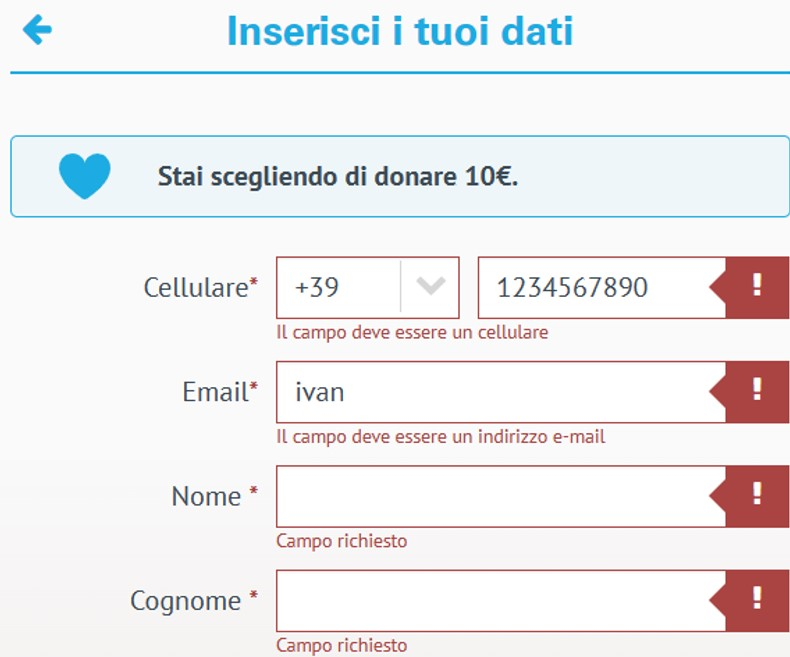
\includegraphics[width=0.5\textwidth]{Picture1.jpg}
		\captionsetup{font=small}
		\caption{\textit{Errors communicated.}}
	\end{center}
\end{figure}
\newline In the 'Contact Us' page, errors are communicated only after the submission of the data (lacking error prevention). Additionally, most of the links on the website have unclear meanings or destinations, potentially leading to errors.
\begin{figure}[!h]
	\begin{center}
		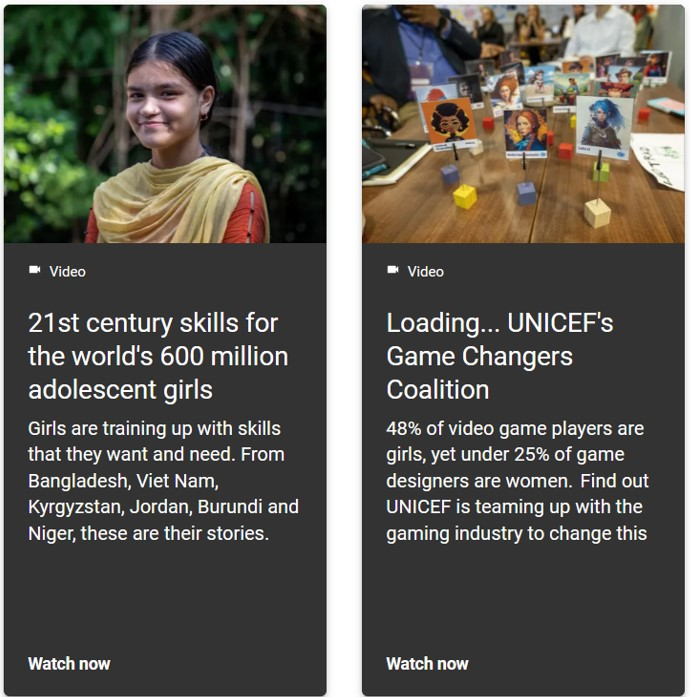
\includegraphics[width=0.4\textwidth]{Picture2.jpg}
		\captionsetup{font=small}
		\caption{\textit{Example of unclear links.}}
	\end{center}
\end{figure}
\newline
\paragraph{H6. Recognition rather than recall - Score 4}	The recognition feature is present when using the search bar, which provides suggestions after entering some characters.
\begin{figure}[!h]
	\begin{center}
		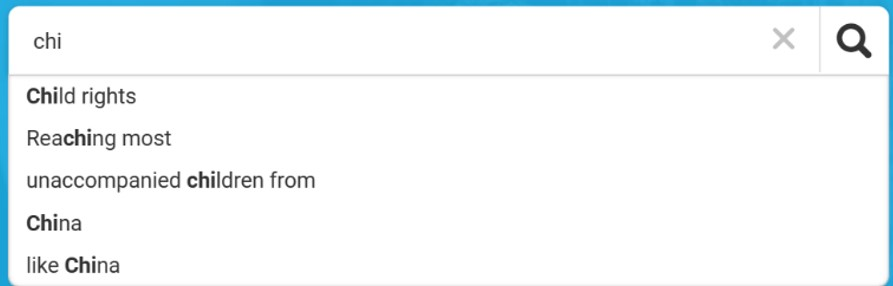
\includegraphics[width=0.5\textwidth]{Picture3.jpg}
		\captionsetup{font=small}
		\caption{\textit{Recognition provided with the search bar.}}
	\end{center}
\end{figure}
\newline The drop-down menu provides a list of options, neatly categorized by topics, facilitating recognition. However, some pages are excessively hidden and challenging to find, even with the search bar (e.g., the Skills4Girls page).
\newline
\paragraph{H7. Flexibility and efficiency of use - Score 2}	Fewer landmarks are available, and some are particularly challenging to locate. Notably, landmarks positioned in the top-right corner of pages and within the footer are less conspicuous, contributing to navigation difficulties.
\begin{figure}[!h]
	\begin{center}
		
\includegraphics[width=0.4\textwidth]{Picture4.jpg}
		\captionsetup{font=small}
		\caption{\textit{Less visible landmarks.}}
	\end{center}
\end{figure}
\newline
\paragraph{H8. Aesthetic and minimalist design - Score 1}	All the pages of the website feature a large image at the top and are filled with various elements and links that are not necessarily requested by the user, as seen on \href{https://www.unicef.org/gender-equality}{the gender equality page}. This results in a design that is not visually pleasing and lacks a minimalist approach.
\begin{figure}[!h]
	\begin{center}
		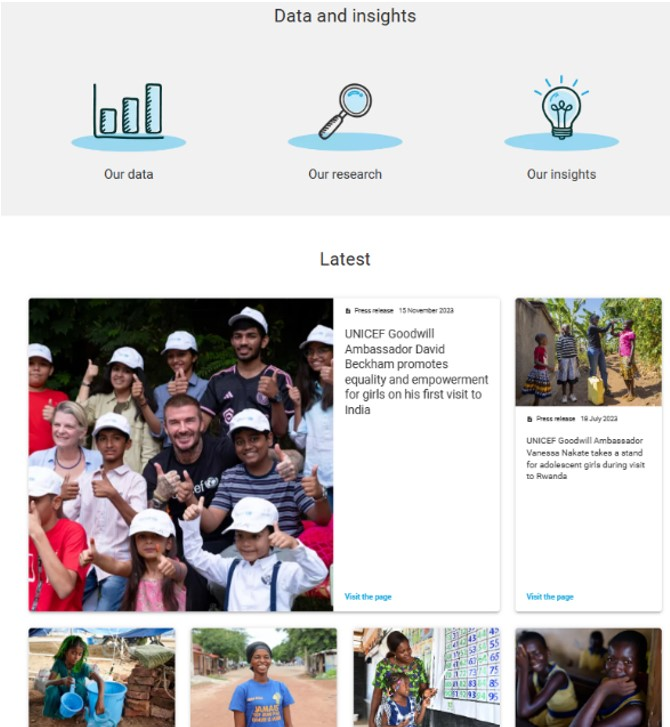
\includegraphics[width=0.5\textwidth]{Picture5.jpg}
		\captionsetup{font=small}
		\caption{\textit{Example of non minimalistic design.}}
	\end{center}
\end{figure}
\newline
\paragraph{H9. Help users recognize, diagnose and recover from errors - Score 5}	Error recognition has a low presence on the website due to its primary focus on articles and fewer features that could lead to errors. However, errors, particularly during the donation process, are adequately identified.
\begin{figure}[!h]
	\begin{center}
		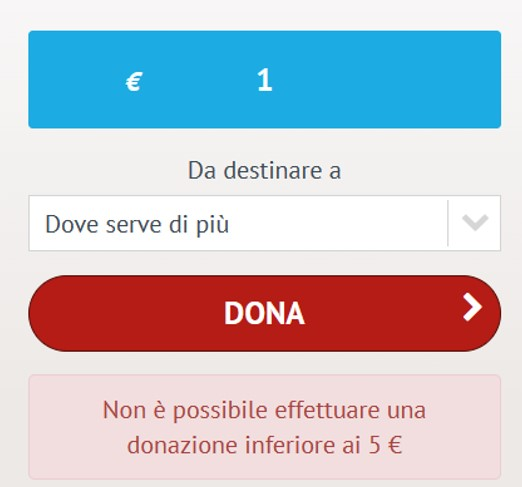
\includegraphics[width=0.3\textwidth]{Picture6.jpg}
		\captionsetup{font=small}
		\caption{\textit{Example of error recognition.}}
	\end{center}
\end{figure}
\newline
\paragraph{H10. Help and documentation - Score 3}	Help and documentation are effectively offered by the FAQ page and the Contact Us page, but they are overly challenging to locate. Specifically, the Contact Us landmark is positioned in the footer and it less visible, the FAQ page is nested within other pages.
\newline
\paragraph{H11. Information overload - Score 1}	In all pages of the website there are very long texts, unnecessary information, and often so many not requested elements are proposed. It’s possible to see all these elements in the \href{https://www.unicef.org/gender-equality}{gender equality page}.
\newline
\paragraph{H12. Consistency of page content structure - Score 3}	The content structure of pages within the same category is not consistently uniform. Some pages with similar topics exhibit varying structures and include different elements, potentially leading to confusion for readers. For instance, on the  \href{https://www.unicef.org/education}{Education page}, there are numerous elements that are typically absent from pages within the same category, these include an unrequested link and a YouTube video positioned in the middle of the page, along with other unnecessary elements.
\begin{figure}[!h]
	\begin{center}
		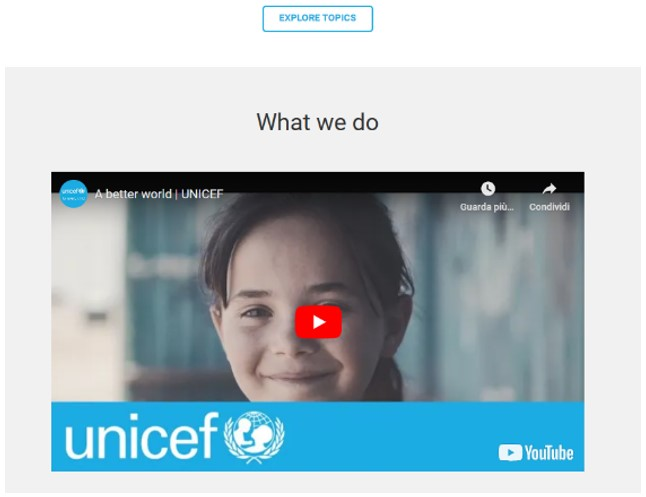
\includegraphics[width=0.45\textwidth]{Picture7.jpg}
		\captionsetup{font=small}
		\caption{\textit{ An unrequested link and a YouTube video in the middle of the page.}}
	\end{center}
\end{figure}
\begin{figure}[!h]
	\begin{center}
		
\includegraphics[width=0.45\textwidth]{Picture8.jpg}
		\captionsetup{font=small}
		\caption{\textit{Other unnecessary elements.}}
	\end{center}
\end{figure}
\newline
\paragraph{H13. Contextualized information - Score 4}	There are some elements that help users to understand where they are, and so to contextualize information, for example in all pages there are images related to the topic, and also the title of each page helps users in this sense. Nevertheless it could be done better with consistent breadcrumbs in each page.
\begin{figure}[!h]
	\begin{center}
		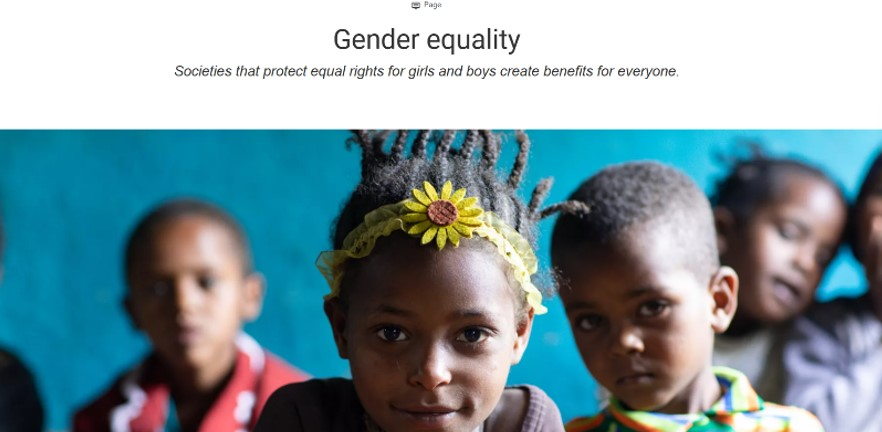
\includegraphics[width=0.6\textwidth]{Picture9.jpg}
		\captionsetup{font=small}
		\caption{\textit{A title and an image which contextualize information.}}
	\end{center}
\end{figure}
\newline
\paragraph{H14. Content organisation (hierarchy) - Score 4}	The hierarchy of some topics is structured on a single page, while others have a well-defined hierarchy spread across multiple pages, featuring few levels with a significant amount of content at each level. For example, the hierarchy of the contents related to child rights exhibits this structure.
\newline Overall, this hierarchical organization is suitable for the topics covered on the website. However, the large number of topics can make the entire hierarchy somewhat confusing for users to navigate.
\begin{figure}[!h]
	\begin{center}
		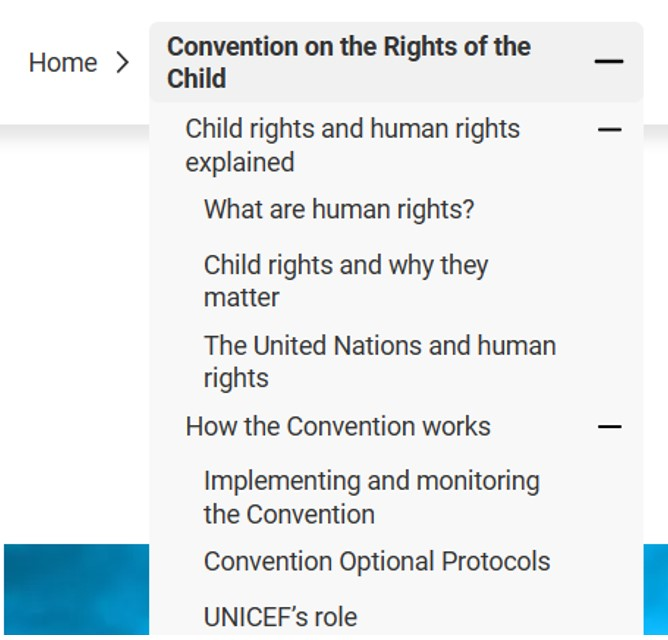
\includegraphics[width=0.4\textwidth]{Picture10.jpg}
		\captionsetup{font=small}
		\caption{\textit{Hierarchy of the 'child rights' topic.}}
	\end{center}
\end{figure}
\newline
\paragraph{H15. Interaction consistency - Score 2}	In terms of navigation links, most pages on the website have consistent menus, at least when the main menu remains unchanged. However, there are numerous pages, acting as subsections, that feature entirely different menus, leading to varying navigation links and causing significant interaction inconsistencies.
\newline For instance, the differences between the menus of the \href{https://www.unicef.org/careers/}{Work with Us} and \href{https://www.unicef.org/partnerships}{Partner with Us} pages illustrate this inconsistency. Generally, it's too easy to open a page with a different menu and become confused due to the inconsistency in navigation.
\newline
\paragraph{H16. Group navigation-1 - Score 3}	The menus group similar items together, making it relatively easy to navigate between and within them. However, these menus are quite large and contain a significant number of elements, which can lead to some confusion for users.
\newline
\paragraph{H17. Group navigation-2 - Score 1}	The big amount of possible links to select in the various drop-down menus can create a lot of confusion in the user, potentially leading to cognitive overload.
\begin{figure}[!h]
	\begin{center}
		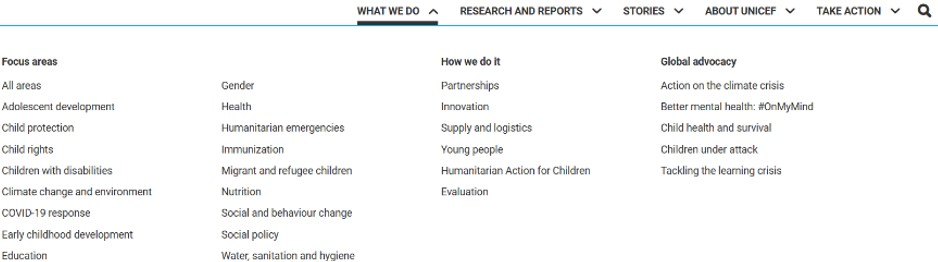
\includegraphics[width=\textwidth]{Picture11.jpg}
		\captionsetup{font=small}
		\caption{\textit{The main menu of the website.}}
	\end{center}
\end{figure}
\newline
\paragraph{H18. Structural navigation - Score 3}	Typically, a single topic is presented on a single page within this website and it relatively easy to navigate among components of that topic. But it is common that after opening a link present on that page, users find it difficult to navigate back, resulting in a bad structural navigation experience.
\newline
\paragraph{H19. Semantic navigation - Score 4}	Usually, similar topics are grouped and linked by a new drop-down menu present at the top of the pages, this makes easy to navigate among related topics in both directions.
\newline But again, if in a page I select a link related to the topic which is not in that menu, usually it’s not possible to go back, so also in this case there are some problems in navigation.
\begin{figure}[!h]
	\begin{center}
		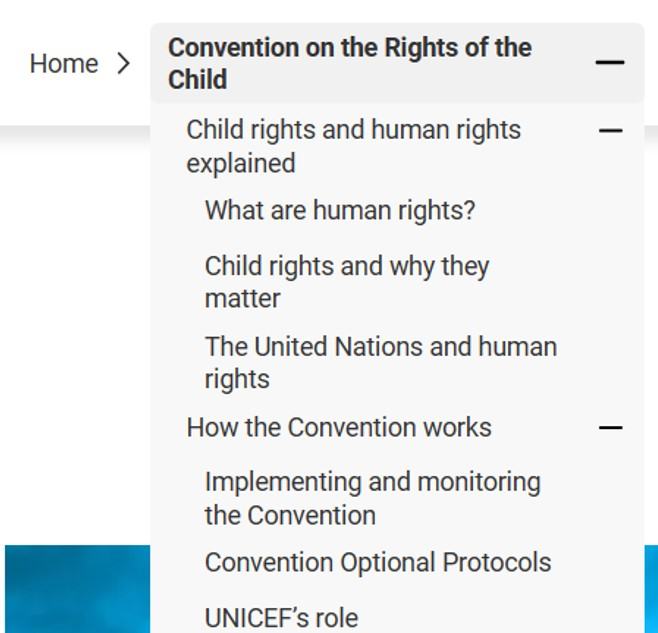
\includegraphics[width=0.4\textwidth]{Picture12.jpg}
		\captionsetup{font=small}
		\caption{\textit{Example of similar topics linked by a drop-down menu.}}
	\end{center}
\end{figure}
\newline
\paragraph{H20. “Landmarks” - Score 2}	
In general, landmarks are not particularly effective because many of them are not very visible. Additionally, there are instances where users may navigate to a different section of the website, causing the destination of the "home" landmark to change.
For example, the "home" landmark on the \href{https://www.unicef.org/careers/}{Work with Us} page does not lead to the true homepage of the website. Instead, a different, less visible and unintuitive landmark is required for this purpose. This inconsistency is observed on other pages as well.
\begin{figure}[!h]
	\begin{center}
		
\includegraphics[width=0.6\textwidth]{Picture13.jpg}
		\captionsetup{font=small}
		\caption{\textit{The new 'home' landamrk.}}
	\end{center}
\end{figure}
\newline
\paragraph{H21. Text lay out - Score 4}	In general, the text is readable and the font size is appropriate. Only few elements are less visible like landmarks showed before.
\newline
\paragraph{H22. Interaction placeholders-semiotics - Score 2}	Not all interactive elements are intuitive. For instance, on all pages, the drop-down menus also function as links, which deviates from the standard menu behavior and can be confusing for users. Moreover, many other links lack clarity regarding their destination or whether they will open a new website.
For example, certain links appear like other normal cards but unexpectedly lead to a YouTube page.
\begin{figure}[!h]
	\begin{center}
		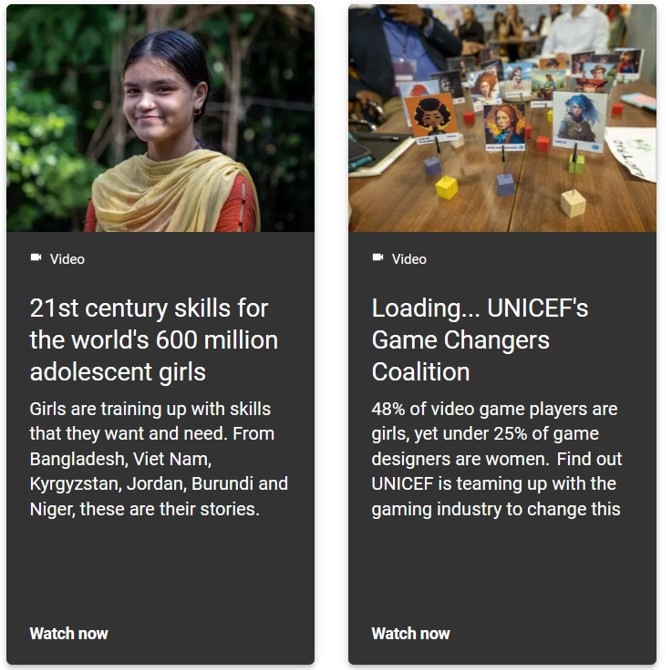
\includegraphics[width=0.4\textwidth]{Picture14.jpg}
		\captionsetup{font=small}
		\caption{\textit{Links that open a YouTube page.}}
	\end{center}
\end{figure}
\newline
\paragraph{H23. Interaction placeholders-consistency - Score 1}	The visual labels of interactive elements are frequently inconsistent. For instance, there are similar interactive elements that are presented in different colours without apparent reason. Another inconsistency pertains to videos; they are not always represented as previously shown but are sometimes integrated directly into the page.
\begin{figure}[!h]
	\begin{center}
		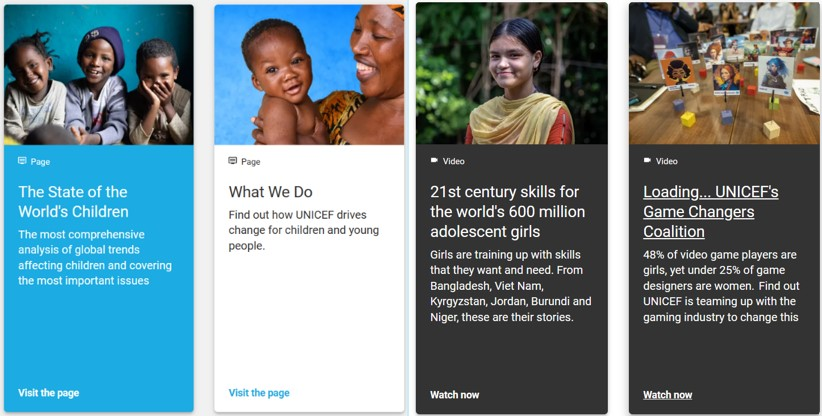
\includegraphics[width=0.6\textwidth]{Picture15.jpg}
		\captionsetup{font=small}
		\caption{\textit{Similar interactive elements with different background colours.}}
	\end{center}
\end{figure}
\begin{figure}[!h]
	\begin{center}
		
\includegraphics[width=0.5\textwidth]{Picture16.jpg}
		\captionsetup{font=small}
		\caption{\textit{A video integrated in a page.}}
	\end{center}
\end{figure}
\newline
\paragraph{H24. Consistency of visual elements - Score 4}	In pages of the same type, visual elements typically share consistent properties, ensuring a level of uniformity. However, certain interactive elements, as illustrated in heuristic 23, exhibit inconsistencies.
\newline
\paragraph{H25. Hierarchy-1 - Score 5}	In my opinion, the hierarchy in a page reflect in accurate way the importance of the contents.
\newline
\paragraph{H26. Hierarchy-2 - Score 5}	The hierarchy of visual elements is fine too.
\newline
\paragraph{H27. Spatial allocation-1 - Score 4}	The 'Contact Us' landmark is expected to be located in the drop-down menu 'About UNICEF' due to their semantic relation, but it is instead placed in the footer, which creates a considerable distance.
On the other hand, for the most part, semantically related elements are sufficiently close to each other.
\newline
\paragraph{H28. Spatial allocation-2 - Score 4}	Semantically distant elements are typically positioned far apart from each other. However, I think the 'Press Centre' button should not be placed at the top-right of the page since it is unrelated to the header and the donate button. Instead, it may be more appropriate to place it within the white bar containing the drop-down menus, where it could be more contextually relevant.
\begin{figure}[!h]
	\begin{center}
		
\includegraphics[width=\textwidth]{Picture17.jpg}
		\captionsetup{font=small}
		\caption{\textit{The header of the website.}}
	\end{center}
\end{figure}
\newline
\paragraph{H29. Consistency of page spatial structure - Score 5}	For the main visual elements, the spatial organization on the page is consistent across pages of the same type.
